% Created by tikzDevice version 0.12.3 on 2020-04-21 11:12:08
% !TEX encoding = UTF-8 Unicode
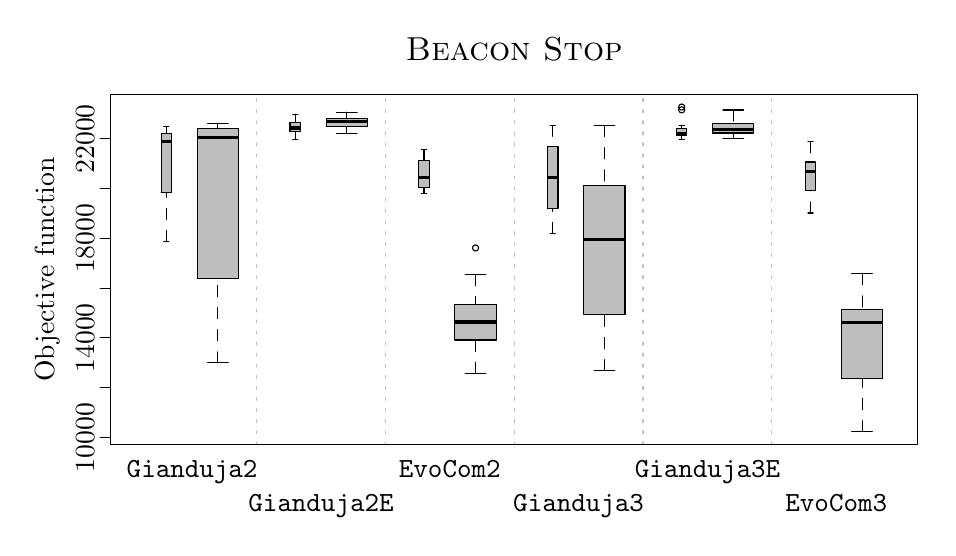
\begin{tikzpicture}[x=1pt,y=1pt]
\definecolor{fillColor}{RGB}{255,255,255}
\path[use as bounding box,fill=fillColor,fill opacity=0.00] (0,0) rectangle (325.21,180.67);
\begin{scope}
\path[clip] ( 30.00, 30.00) rectangle (321.61,156.67);
\definecolor{fillColor}{RGB}{190,190,190}

\path[fill=fillColor] ( 48.25,121.11) --
	( 51.97,121.11) --
	( 51.97,142.47) --
	( 48.25,142.47) --
	cycle;
\definecolor{drawColor}{RGB}{0,0,0}

\path[draw=drawColor,line width= 1.2pt,line join=round] ( 48.25,139.60) -- ( 51.97,139.60);

\path[draw=drawColor,line width= 0.4pt,dash pattern=on 4pt off 4pt ,line join=round,line cap=round] ( 50.11,103.31) -- ( 50.11,121.11);

\path[draw=drawColor,line width= 0.4pt,dash pattern=on 4pt off 4pt ,line join=round,line cap=round] ( 50.11,144.87) -- ( 50.11,142.47);

\path[draw=drawColor,line width= 0.4pt,line join=round,line cap=round] ( 49.18,103.31) -- ( 51.04,103.31);

\path[draw=drawColor,line width= 0.4pt,line join=round,line cap=round] ( 49.18,144.87) -- ( 51.04,144.87);

\path[draw=drawColor,line width= 0.4pt,line join=round,line cap=round] ( 48.25,121.11) --
	( 51.97,121.11) --
	( 51.97,142.47) --
	( 48.25,142.47) --
	( 48.25,121.11);

\path[fill=fillColor] ( 61.28, 90.09) --
	( 76.18, 90.09) --
	( 76.18,144.16) --
	( 61.28,144.16) --
	cycle;

\path[draw=drawColor,line width= 1.2pt,line join=round] ( 61.28,141.07) -- ( 76.18,141.07);

\path[draw=drawColor,line width= 0.4pt,dash pattern=on 4pt off 4pt ,line join=round,line cap=round] ( 68.73, 59.53) -- ( 68.73, 90.09);

\path[draw=drawColor,line width= 0.4pt,dash pattern=on 4pt off 4pt ,line join=round,line cap=round] ( 68.73,146.04) -- ( 68.73,144.16);

\path[draw=drawColor,line width= 0.4pt,line join=round,line cap=round] ( 65.01, 59.53) -- ( 72.46, 59.53);

\path[draw=drawColor,line width= 0.4pt,line join=round,line cap=round] ( 65.01,146.04) -- ( 72.46,146.04);

\path[draw=drawColor,line width= 0.4pt,line join=round,line cap=round] ( 61.28, 90.09) --
	( 76.18, 90.09) --
	( 76.18,144.16) --
	( 61.28,144.16) --
	( 61.28, 90.09);

\path[fill=fillColor] ( 94.80,143.06) --
	( 98.53,143.06) --
	( 98.53,146.42) --
	( 94.80,146.42) --
	cycle;

\path[draw=drawColor,line width= 1.2pt,line join=round] ( 94.80,144.44) -- ( 98.53,144.44);

\path[draw=drawColor,line width= 0.4pt,dash pattern=on 4pt off 4pt ,line join=round,line cap=round] ( 96.67,140.36) -- ( 96.67,143.06);

\path[draw=drawColor,line width= 0.4pt,dash pattern=on 4pt off 4pt ,line join=round,line cap=round] ( 96.67,149.38) -- ( 96.67,146.42);

\path[draw=drawColor,line width= 0.4pt,line join=round,line cap=round] ( 95.73,140.36) -- ( 97.60,140.36);

\path[draw=drawColor,line width= 0.4pt,line join=round,line cap=round] ( 95.73,149.38) -- ( 97.60,149.38);

\path[draw=drawColor,line width= 0.4pt,line join=round,line cap=round] ( 94.80,143.06) --
	( 98.53,143.06) --
	( 98.53,146.42) --
	( 94.80,146.42) --
	( 94.80,143.06);

\path[fill=fillColor] (107.84,145.00) --
	(122.74,145.00) --
	(122.74,147.76) --
	(107.84,147.76) --
	cycle;

\path[draw=drawColor,line width= 1.2pt,line join=round] (107.84,146.79) -- (122.74,146.79);

\path[draw=drawColor,line width= 0.4pt,dash pattern=on 4pt off 4pt ,line join=round,line cap=round] (115.29,142.34) -- (115.29,145.00);

\path[draw=drawColor,line width= 0.4pt,dash pattern=on 4pt off 4pt ,line join=round,line cap=round] (115.29,150.16) -- (115.29,147.76);

\path[draw=drawColor,line width= 0.4pt,line join=round,line cap=round] (111.56,142.34) -- (119.01,142.34);

\path[draw=drawColor,line width= 0.4pt,line join=round,line cap=round] (111.56,150.16) -- (119.01,150.16);

\path[draw=drawColor,line width= 0.4pt,line join=round,line cap=round] (107.84,145.00) --
	(122.74,145.00) --
	(122.74,147.76) --
	(107.84,147.76) --
	(107.84,145.00);

\path[fill=fillColor] (141.36,122.87) --
	(145.08,122.87) --
	(145.08,132.71) --
	(141.36,132.71) --
	cycle;

\path[draw=drawColor,line width= 1.2pt,line join=round] (141.36,126.45) -- (145.08,126.45);

\path[draw=drawColor,line width= 0.4pt,dash pattern=on 4pt off 4pt ,line join=round,line cap=round] (143.22,120.82) -- (143.22,122.87);

\path[draw=drawColor,line width= 0.4pt,dash pattern=on 4pt off 4pt ,line join=round,line cap=round] (143.22,136.64) -- (143.22,132.71);

\path[draw=drawColor,line width= 0.4pt,line join=round,line cap=round] (142.29,120.82) -- (144.15,120.82);

\path[draw=drawColor,line width= 0.4pt,line join=round,line cap=round] (142.29,136.64) -- (144.15,136.64);

\path[draw=drawColor,line width= 0.4pt,line join=round,line cap=round] (141.36,122.87) --
	(145.08,122.87) --
	(145.08,132.71) --
	(141.36,132.71) --
	(141.36,122.87);

\path[fill=fillColor] (154.39, 67.80) --
	(169.29, 67.80) --
	(169.29, 80.60) --
	(154.39, 80.60) --
	cycle;

\path[draw=drawColor,line width= 1.2pt,line join=round] (154.39, 74.27) -- (169.29, 74.27);

\path[draw=drawColor,line width= 0.4pt,dash pattern=on 4pt off 4pt ,line join=round,line cap=round] (161.84, 55.69) -- (161.84, 67.80);

\path[draw=drawColor,line width= 0.4pt,dash pattern=on 4pt off 4pt ,line join=round,line cap=round] (161.84, 91.46) -- (161.84, 80.60);

\path[draw=drawColor,line width= 0.4pt,line join=round,line cap=round] (158.12, 55.69) -- (165.57, 55.69);

\path[draw=drawColor,line width= 0.4pt,line join=round,line cap=round] (158.12, 91.46) -- (165.57, 91.46);

\path[draw=drawColor,line width= 0.4pt,line join=round,line cap=round] (154.39, 67.80) --
	(169.29, 67.80) --
	(169.29, 80.60) --
	(154.39, 80.60) --
	(154.39, 67.80);

\path[draw=drawColor,line width= 0.4pt,line join=round,line cap=round] (161.84,101.08) circle (  1.12);

\path[fill=fillColor] (187.91,115.25) --
	(191.64,115.25) --
	(191.64,137.57) --
	(187.91,137.57) --
	cycle;

\path[draw=drawColor,line width= 1.2pt,line join=round] (187.91,126.65) -- (191.64,126.65);

\path[draw=drawColor,line width= 0.4pt,dash pattern=on 4pt off 4pt ,line join=round,line cap=round] (189.77,106.29) -- (189.77,115.25);

\path[draw=drawColor,line width= 0.4pt,dash pattern=on 4pt off 4pt ,line join=round,line cap=round] (189.77,145.38) -- (189.77,137.57);

\path[draw=drawColor,line width= 0.4pt,line join=round,line cap=round] (188.84,106.29) -- (190.70,106.29);

\path[draw=drawColor,line width= 0.4pt,line join=round,line cap=round] (188.84,145.38) -- (190.70,145.38);

\path[draw=drawColor,line width= 0.4pt,line join=round,line cap=round] (187.91,115.25) --
	(191.64,115.25) --
	(191.64,137.57) --
	(187.91,137.57) --
	(187.91,115.25);

\path[fill=fillColor] (200.95, 77.08) --
	(215.84, 77.08) --
	(215.84,123.51) --
	(200.95,123.51) --
	cycle;

\path[draw=drawColor,line width= 1.2pt,line join=round] (200.95,104.24) -- (215.84,104.24);

\path[draw=drawColor,line width= 0.4pt,dash pattern=on 4pt off 4pt ,line join=round,line cap=round] (208.40, 56.74) -- (208.40, 77.08);

\path[draw=drawColor,line width= 0.4pt,dash pattern=on 4pt off 4pt ,line join=round,line cap=round] (208.40,145.28) -- (208.40,123.51);

\path[draw=drawColor,line width= 0.4pt,line join=round,line cap=round] (204.67, 56.74) -- (212.12, 56.74);

\path[draw=drawColor,line width= 0.4pt,line join=round,line cap=round] (204.67,145.28) -- (212.12,145.28);

\path[draw=drawColor,line width= 0.4pt,line join=round,line cap=round] (200.95, 77.08) --
	(215.84, 77.08) --
	(215.84,123.51) --
	(200.95,123.51) --
	(200.95, 77.08);

\path[fill=fillColor] (234.47,141.74) --
	(238.19,141.74) --
	(238.19,144.31) --
	(234.47,144.31) --
	cycle;

\path[draw=drawColor,line width= 1.2pt,line join=round] (234.47,142.40) -- (238.19,142.40);

\path[draw=drawColor,line width= 0.4pt,dash pattern=on 4pt off 4pt ,line join=round,line cap=round] (236.33,140.36) -- (236.33,141.74);

\path[draw=drawColor,line width= 0.4pt,dash pattern=on 4pt off 4pt ,line join=round,line cap=round] (236.33,145.40) -- (236.33,144.31);

\path[draw=drawColor,line width= 0.4pt,line join=round,line cap=round] (235.40,140.36) -- (237.26,140.36);

\path[draw=drawColor,line width= 0.4pt,line join=round,line cap=round] (235.40,145.40) -- (237.26,145.40);

\path[draw=drawColor,line width= 0.4pt,line join=round,line cap=round] (234.47,141.74) --
	(238.19,141.74) --
	(238.19,144.31) --
	(234.47,144.31) --
	(234.47,141.74);

\path[draw=drawColor,line width= 0.4pt,line join=round,line cap=round] (236.33,150.98) circle (  1.12);

\path[draw=drawColor,line width= 0.4pt,line join=round,line cap=round] (236.33,151.98) circle (  1.12);

\path[fill=fillColor] (247.50,142.59) --
	(262.40,142.59) --
	(262.40,145.92) --
	(247.50,145.92) --
	cycle;

\path[draw=drawColor,line width= 1.2pt,line join=round] (247.50,143.93) -- (262.40,143.93);

\path[draw=drawColor,line width= 0.4pt,dash pattern=on 4pt off 4pt ,line join=round,line cap=round] (254.95,140.78) -- (254.95,142.59);

\path[draw=drawColor,line width= 0.4pt,dash pattern=on 4pt off 4pt ,line join=round,line cap=round] (254.95,150.90) -- (254.95,145.92);

\path[draw=drawColor,line width= 0.4pt,line join=round,line cap=round] (251.23,140.78) -- (258.67,140.78);

\path[draw=drawColor,line width= 0.4pt,line join=round,line cap=round] (251.23,150.90) -- (258.67,150.90);

\path[draw=drawColor,line width= 0.4pt,line join=round,line cap=round] (247.50,142.59) --
	(262.40,142.59) --
	(262.40,145.92) --
	(247.50,145.92) --
	(247.50,142.59);

\path[fill=fillColor] (281.02,121.86) --
	(284.74,121.86) --
	(284.74,132.11) --
	(281.02,132.11) --
	cycle;

\path[draw=drawColor,line width= 1.2pt,line join=round] (281.02,128.66) -- (284.74,128.66);

\path[draw=drawColor,line width= 0.4pt,dash pattern=on 4pt off 4pt ,line join=round,line cap=round] (282.88,113.71) -- (282.88,121.86);

\path[draw=drawColor,line width= 0.4pt,dash pattern=on 4pt off 4pt ,line join=round,line cap=round] (282.88,139.48) -- (282.88,132.11);

\path[draw=drawColor,line width= 0.4pt,line join=round,line cap=round] (281.95,113.71) -- (283.81,113.71);

\path[draw=drawColor,line width= 0.4pt,line join=round,line cap=round] (281.95,139.48) -- (283.81,139.48);

\path[draw=drawColor,line width= 0.4pt,line join=round,line cap=round] (281.02,121.86) --
	(284.74,121.86) --
	(284.74,132.11) --
	(281.02,132.11) --
	(281.02,121.86);

\path[fill=fillColor] (294.05, 53.78) --
	(308.95, 53.78) --
	(308.95, 78.81) --
	(294.05, 78.81) --
	cycle;

\path[draw=drawColor,line width= 1.2pt,line join=round] (294.05, 74.17) -- (308.95, 74.17);

\path[draw=drawColor,line width= 0.4pt,dash pattern=on 4pt off 4pt ,line join=round,line cap=round] (301.50, 34.69) -- (301.50, 53.78);

\path[draw=drawColor,line width= 0.4pt,dash pattern=on 4pt off 4pt ,line join=round,line cap=round] (301.50, 91.73) -- (301.50, 78.81);

\path[draw=drawColor,line width= 0.4pt,line join=round,line cap=round] (297.78, 34.69) -- (305.23, 34.69);

\path[draw=drawColor,line width= 0.4pt,line join=round,line cap=round] (297.78, 91.73) -- (305.23, 91.73);

\path[draw=drawColor,line width= 0.4pt,line join=round,line cap=round] (294.05, 53.78) --
	(308.95, 53.78) --
	(308.95, 78.81) --
	(294.05, 78.81) --
	(294.05, 53.78);
\definecolor{drawColor}{RGB}{190,190,190}

\path[draw=drawColor,line width= 0.4pt,dash pattern=on 1pt off 3pt ,line join=round,line cap=round] ( 82.70, 30.00) -- ( 82.70,156.67);

\path[draw=drawColor,line width= 0.4pt,dash pattern=on 1pt off 3pt ,line join=round,line cap=round] (129.25, 30.00) -- (129.25,156.67);

\path[draw=drawColor,line width= 0.4pt,dash pattern=on 1pt off 3pt ,line join=round,line cap=round] (175.81, 30.00) -- (175.81,156.67);

\path[draw=drawColor,line width= 0.4pt,dash pattern=on 1pt off 3pt ,line join=round,line cap=round] (222.36, 30.00) -- (222.36,156.67);

\path[draw=drawColor,line width= 0.4pt,dash pattern=on 1pt off 3pt ,line join=round,line cap=round] (268.92, 30.00) -- (268.92,156.67);
\end{scope}
\begin{scope}
\path[clip] (  0.00,  0.00) rectangle (325.21,180.67);
\definecolor{drawColor}{RGB}{0,0,0}

\node[text=drawColor,anchor=base,inner sep=0pt, outer sep=0pt, scale=  1.00] at ( 59.42, 18.00) {\texttt{Gianduja2}};

\node[text=drawColor,anchor=base,inner sep=0pt, outer sep=0pt, scale=  1.00] at (152.53, 18.00) {\texttt{EvoCom2}};

\node[text=drawColor,anchor=base,inner sep=0pt, outer sep=0pt, scale=  1.00] at (245.64, 18.00) {\texttt{Gianduja3E}};

\node[text=drawColor,anchor=base,inner sep=0pt, outer sep=0pt, scale=  1.00] at (105.98,  6.00) {\texttt{Gianduja2E}};

\node[text=drawColor,anchor=base,inner sep=0pt, outer sep=0pt, scale=  1.00] at (199.08,  6.00) {\texttt{Gianduja3}};

\node[text=drawColor,anchor=base,inner sep=0pt, outer sep=0pt, scale=  1.00] at (292.19,  6.00) {\texttt{EvoCom3}};
\end{scope}
\begin{scope}
\path[clip] (  0.00,  0.00) rectangle (325.21,180.67);
\definecolor{drawColor}{RGB}{0,0,0}

\node[text=drawColor,anchor=base,inner sep=0pt, outer sep=0pt, scale=  1.20] at (175.81,168.67) {\textsc{Beacon Stop}};

\node[text=drawColor,rotate= 90.00,anchor=base,inner sep=0pt, outer sep=0pt, scale=  1.00] at (  9.60, 93.34) {Objective function};
\end{scope}
\begin{scope}
\path[clip] (  0.00,  0.00) rectangle (325.21,180.67);
\definecolor{drawColor}{RGB}{0,0,0}

\path[draw=drawColor,line width= 0.4pt,line join=round,line cap=round] ( 30.00, 32.61) -- ( 30.00,140.51);

\path[draw=drawColor,line width= 0.4pt,line join=round,line cap=round] ( 30.00, 32.61) -- ( 26.20, 32.61);

\path[draw=drawColor,line width= 0.4pt,line join=round,line cap=round] ( 30.00, 50.59) -- ( 26.20, 50.59);

\path[draw=drawColor,line width= 0.4pt,line join=round,line cap=round] ( 30.00, 68.57) -- ( 26.20, 68.57);

\path[draw=drawColor,line width= 0.4pt,line join=round,line cap=round] ( 30.00, 86.56) -- ( 26.20, 86.56);

\path[draw=drawColor,line width= 0.4pt,line join=round,line cap=round] ( 30.00,104.54) -- ( 26.20,104.54);

\path[draw=drawColor,line width= 0.4pt,line join=round,line cap=round] ( 30.00,122.53) -- ( 26.20,122.53);

\path[draw=drawColor,line width= 0.4pt,line join=round,line cap=round] ( 30.00,140.51) -- ( 26.20,140.51);

\node[text=drawColor,rotate= 90.00,anchor=base,inner sep=0pt, outer sep=0pt, scale=  1.00] at ( 24.00, 32.61) {10000};

\node[text=drawColor,rotate= 90.00,anchor=base,inner sep=0pt, outer sep=0pt, scale=  1.00] at ( 24.00, 68.57) {14000};

\node[text=drawColor,rotate= 90.00,anchor=base,inner sep=0pt, outer sep=0pt, scale=  1.00] at ( 24.00,104.54) {18000};

\node[text=drawColor,rotate= 90.00,anchor=base,inner sep=0pt, outer sep=0pt, scale=  1.00] at ( 24.00,140.51) {22000};

\path[draw=drawColor,line width= 0.4pt,line join=round,line cap=round] ( 30.00, 30.00) --
	(321.61, 30.00) --
	(321.61,156.67) --
	( 30.00,156.67) --
	( 30.00, 30.00);
\end{scope}
\end{tikzpicture}
